\documentclass[12pt]{article}
\usepackage{amsmath}
\usepackage{graphicx}
\usepackage{hyperref}
\usepackage{listings}
\usepackage{color}
\usepackage{pythonhighlight}

\title{Operating System Course Report - First Half of the Semester}
\author{A class}
\date{\today}

\begin{document}

\maketitle
\newpage

\tableofcontents
\newpage

\section{Introduction}
This report summarizes the topics covered during the first half of the Operating System course. It includes theoretical concepts, practical implementations, and assignments. The course focuses on the fundamentals of operating systems, including system architecture, process management, CPU scheduling, and deadlock handling.

\section{Course Overview}
\subsection{Objectives}
The main objectives of this course are:
\begin{itemize}
    \item To understand the basic components and architecture of a computer system.
    \item To learn process management, scheduling, and inter-process communication.
    \item To explore file systems, input/output management, and virtualization.
    \item To study the prevention and handling of deadlocks in operating systems.
\end{itemize}

\subsection{Course Structure}
The course is divided into two halves. This report focuses on the first half, which covers:
\begin{itemize}
    \item Basic Concepts and Components of Computer Systems
    \item System Performance and Metrics
    \item System Architecture of Computer Systems
    \item Process Description and Control
    \item Scheduling Algorithms
    \item Process Creation and Termination
    \item Introduction to Threads
    \item File Systems
    \item Input and Output Management
    \item Deadlock Introduction and Prevention
    \item User Interface Management
    \item Virtualization in Operating Systems
\end{itemize}

\section{Topics Covered}

\subsection{Basic Concepts and Components of Computer Systems}
This section explains the fundamental components that make up a computer system, including the CPU, memory, storage, and input/output devices.

\subsection{System Performance and Metrics}
This section introduces various system performance metrics used to measure the efficiency of a computer system, including throughput, response time, and utilization.

\subsection{System Architecture of Computer Systems}
Describes the architecture of modern computer systems, focusing on the interaction between hardware and the operating system.

\subsection{Process Description and Control}
Processes are a central concept in operating systems. This section covers:
\begin{itemize}
    \item Process states and state transitions
    \item Process control block (PCB)
    \item Context switching
\end{itemize}

\subsection{Scheduling Algorithms}
This section covers:
\begin{itemize}
    \item First-Come, First-Served (FCFS)
    \item Shortest Job Next (SJN)
    \item Round Robin (RR)
\end{itemize}
It explains how these algorithms are used to allocate CPU time to processes.

\subsection{Process Creation and Termination}
Details how processes are created and terminated by the operating system, including:
\begin{itemize}
    \item Process spawning
    \item Process termination conditions
\end{itemize}

\subsection{Introduction to Threads}
This section introduces the concept of threads and their relation to processes, covering:
\begin{itemize}
    \item Single-threaded vs. multi-threaded processes
    \item Benefits of multithreading
\end{itemize}

\begin{figure}[h]
    \centering
    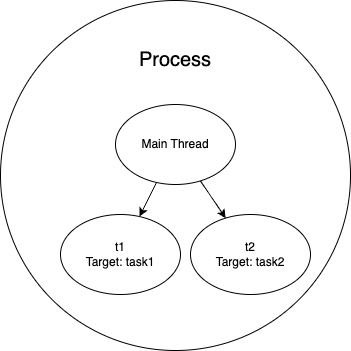
\includegraphics[width=0.5\textwidth]{/Users/khawaritzmi/Unhas/os_report_mid2024/a_class/asset/example.png}  % Sesuaikan nama file dan ukurannya
    \caption{Ini adalah gambar contoh dari multithreading.}
    \label{fig:contoh_gambar}
\end{figure}

Seperti yang terlihat pada Gambar \ref{fig:contoh_gambar}, inilah cara menambahkan gambar dengan keterangan.

\subsection{File Systems}
File systems provide a way for the operating system to store, retrieve, and manage data. This section explains:
\begin{itemize}
    \item File system structure
    \item File access methods
    \item Directory management
\end{itemize}
\textbf{Sintasi:} Zettagrid. (2024, April 2) menjelaskan pengertian, manfaat dan metode hingga keamanan \textit{file sharing}, sebagai berikut:
\item \textbf{\textit{File Sharing}} adalah proses yang memungkinkan individu atau entitas untuk berbagi \textit{file} digital dengan orang lain melalui jaringan komputer atau internet. Ini memungkinkan pengguna untuk mentransfer \textit{file}, seperti dokumen, gambar, video, musik, dan lainnya, dari satu perangkat ke perangkat lainnya. \textit{File sharing} dapat dilakukan secara lokal, melalui jaringan lokal seperti LAN (\textit{Local Area Network}), atau secara \textit{online} melalui layanan\textit{ cloud} atau platform \textit{file sharing} .
\begin{itemize}
    \item {Manfaat File Sharing} 
    
    Dalam era digital saat ini, dimana kolaborasi dan pertukaran informasi menjadi kunci kesuksesan, praktik \textit{file sharing} telah menjadi salah satu aspek terpenting dalam berbagai lingkungan kerja. Baik itu dalam tim kecil, perusahaan besar, atau bahkan dalam lingkup pendidikan, kemampuan untuk berbagi \textit{file} dengan cepat dan efisien telah menjadi landasan dari produktivitas dan inovasi.
    Berikut manfaat penting \textit{file sharing} dalam meningkatkan efisiensi dan kolaborasi di lingkungan kerja modern:
    \begin{itemize}
       \item Akses Mudah dan Cepat 
       
        Salah satu keuntungan utama dari \textit{file sharing} adalah akses mudah dan cepat terhadap informasi. Dengan menggunakan platform\textit{ file sharing} yang tepat, seperti Google Drive, Dropbox, atau OneDrive, individu atau tim dapat dengan mudah mengunggah dan mengunduh file dari mana saja, kapan saja, asalkan terhubung ke internet. Ini memungkinkan anggota tim untuk mengakses dokumen penting bahkan saat mereka tidak berada di kantor atau di lokasi fisik lainnya.
        \item Kolaborasi Tim yang Efisien

        \textit{File sharing} juga memainkan peran kunci dalam memfasilitasi kolaborasi tim yang efisien. Dengan berbagi \textit{file }secara \textit{online}, anggota tim dapat secara bersama-sama mengedit dokumen, menyampaikan umpan balik, dan melacak perubahan dalam waktu nyata. Ini menghilangkan kebutuhan untuk mengirim \textit{file} melalui email atau menyimpan versi terbaru secara terpisah, yang sering kali dapat mengakibatkan kekacauan dan kebingungan.
       \item Peningkatan Produktivitas 

       Dengan akses mudah dan kolaborasi yang ditingkatkan, \textit{file sharing} berkontribusi secara langsung pada peningkatan produktivitas di tempat kerja. Tim dapat bekerja lebih efisien, menghemat waktu yang sebelumnya dihabiskan untuk mencari \textit{file} yang diperlukan atau menunggu tanggapan dari rekan kerja. Selain itu, dengan kemampuan untuk mengakses \textit{file} dari berbagai perangkat, seperti laptop, tablet, atau ponsel pintar, individu dapat tetap produktif bahkan saat mereka berada dalam perjalanan.
       \item Backup dan Penyimpanan
       
       Meskipun kemudahan akses dan kolaborasi yang ditawarkan oleh \textit{file sharing} sangatlah penting, keamanan data juga merupakan faktor yang tidak boleh diabaikan. \textit{Platform file sharing} modern sering dilengkapi dengan fitur keamanan canggih, seperti enkripsi end-to-end, kontrol akses, dan otorisasi dua faktor, yang membantu melindungi informasi sensitif dari akses yang tidak sah atau kebocoran data. Ini memberikan ketenangan pikiran kepada organisasi bahwa data mereka aman, bahkan saat berada dalam perjalanan di internet.
       \vspace{2pt}
    \end{itemize}
    \item Metode File Sharing

    \textit{File sharing} adalah praktik yang memungkinkan individu atau organisasi untuk berbagi data dengan mudah dan efisien. Dalam dunia digital saat ini, terdapat berbagai metode yang dapat digunakan untuk melakukan \textit{file sharing}, masing-masing dengan kelebihan dan kekurangan. Berikut adalah beberapa metode \textit{file sharing} yang umum digunakan:

    \begin{itemize}
        \item Layanan \textit{Cloud Storage}

        Email masih menjadi salah satu cara yang paling umum digunakan untuk berbagi \textit{file}. Pengguna dapat melampirkan \textit{file} ke pesan email dan mengirimkannya kepada penerima yang diinginkan. Sebagian besar penyedia layanan email memiliki batasan ukuran \textit{file} yang dapat dilampirkan, jadi pastikan ukuran \textit{file} tidak melebihi batas yang ditetapkan.
        \item Aplikasi P2P (\textit{Peer-to-Peer})

        Aplikasi P2P memungkinkan pengguna untuk berbagi \textit{file} langsung antara satu sama lain, tanpa perantara. Pengguna menggunakan perangkat lunak khusus untuk terhubung ke jaringan P2P dan dapat mengunduh atau mengunggah\textit{ file} sesuai kebutuhan.
        
        \item Tautan Berbagi

        Banyak \textit{platform file sharing,} termasuk layanan penyimpanan awan dan platform kolaborasi seperti Google Drive dan SharePoint, memungkinkan pengguna untuk membuat tautan berbagi yang dapat dibagikan kepada orang lain. Dengan mengirimkan tautan ini, penerima dapat mengakses \textit{file} tanpa perlu \textit{log in} atau memiliki akun di \textit{platform} tersebut.
        \item Jaringan Lokal (LAN)

        \textit{File sharing} menggunakan jaringan lokal (LAN) memungkinkan berbagi \textit{file} antar perangkat yang terhubung dalam jaringan internal tanpa memerlukan internet. Ini bisa dilakukan dengan berbagai metode, seperti berbagi folder di Windows atau Mac, menggunakan perangkat \textit{Network Attached Storage} (NAS), atau melalui protokol SMB dan FTP. Metode ini memberikan kecepatan transfer yang tinggi, mudah diakses, dan cocok untuk kolaborasi dalam organisasi kecil seperti kantor atau sekolah. Namun, penting untuk memastikan keamanan dengan mengatur izin akses dan menjaga jaringan dari ancaman eksternal.
    \end{itemize}
      \textbf{  Sintasi:} Filemail. (n.d.) menjelaskan keamanan dalam \textit{file sharing}, sebagai berikut;
    \item Keamanan dalam \textit{File Sharing}
    
    Keamanan dalam \textit{file sharing} sangat penting untuk menjaga data dari akses tidak sah, pencurian informasi, atau penyebaran \textit{malware}. \textit{File sharing} yang tidak dilindungi dengan baik dapat menjadi target serangan siber, yang berisiko menyebabkan kerugian besar, terutama bagi organisasi yang menangani informasi sensitif. Untuk itu, beberapa langkah dapat diambil guna memastikan bahwa \textit{file sharing} dilakukan dengan aman.
    \begin{itemize}
        \item Enkripsi File

        Enkripsi \textit{file} adalah proses mengamankan data sehingga hanya pengguna yang memiliki kunci enkripsi yang dapat membukanya. Enkripsi melindungi\textit{ file }selama penyimpanan \textit{(at rest)} dan saat dikirim \textit{(in transit)}. Ketika \textit{file} dibagikan melalui internet atau jaringan, enkripsi memastikan bahwa meskipun \textit{file} tersebut dicegat oleh pihak yang tidak sah, isinya tidak dapat dibaca tanpa kunci yang sesuai.
        \item Izin Akses

        Izin akses bertujuan untuk mengatur siapa saja yang dapat melihat, mengedit, atau menghapus \textit{file}. Ini penting untuk membatasi akses hanya kepada pengguna yang berwenang. Dengan membatasi hak akses, organisasi dapat menghindari potensi penyalahgunaan \textit{file} oleh pengguna yang tidak berhak.

        \item Autentikasi dan Kata Sandi

        Autentikasi yang kuat dan penggunaan kata sandi yang kompleks sangat penting dalam menjaga keamanan \textit{file sharing}. Autentikasi dapat dilakukan dengan memverifikasi identitas pengguna melalui metode seperti autentikasi dua faktor (2FA). Kata sandi yang kompleks dan unik mengurangi risiko peretasan yang sering terjadi akibat kata sandi yang lemah.

        \item \textit{Firewall} dan Antivirus

        \textit{Firewall} berfungsi sebagai pelindung terhadap akses tidak sah ke dalam jaringan, sementara antivirus melindungi perangkat dari serangan \textit{malware}. Mengaktifkan \textit{firewall} dan memastikan antivirus selalu diperbarui adalah cara untuk mencegah serangan siber yang dapat mencuri atau merusak \textit{file }selama proses \textit{sharing}.

        \item VPN (\textit{Virtual Private Network})

        VPN digunakan untuk mengenkripsi koneksi jaringan saat berbagi \textit{file }jarak jauh melalui internet. VPN melindungi data dari penyadapan dengan mengenkripsi seluruh lalu lintas jaringan yang melewati \textit{server}. Hal ini memastikan bahwa \textit{file} yang dikirim tidak dapat dilihat oleh pihak ketiga selama proses \textit{transfer}.
    \end{itemize}
\end{itemize}

\begin{thebibliography}{99}
        \bibitem{sharing}
        Zettagrid. (2024, April 2). \textit{File sharing: Pengertian, manfaat, dan metode file sharing dengan mudah}. Diambil dari https://www.zettagrid.id/blog/2024/04/02/file-sharing-pengertian-manfaat-dan-metode-file-sharing-dengan-mudah/
        \bibitem{keamanan}
        Filemail. (n.d.). \textit{Apa itu berbagi file? Bagaimana cara kerjanya.} Diambil dari https://www.filemail.com/id/blog/berbagi-file/apa-itu-berbagi-file-bagaimana-cara-kerjanya
    \end{thebibliography}


\subsection{Input and Output Management}
Input and output management is key for handling the interaction between the system and external devices. This section includes:
\begin{itemize}
    \item Device drivers
    \item I/O scheduling
\end{itemize}

\subsection{Deadlock Introduction and Prevention}
Explores the concept of deadlocks and methods for preventing them:
\begin{itemize}
    \item Deadlock conditions
    \item Deadlock prevention techniques
\end{itemize}

\subsection{User Interface Management}
This section discusses the role of the operating system in managing the user interface. Topics covered include:
\begin{itemize}
    \item Graphical User Interface (GUI)
    \item Command-Line Interface (CLI)
    \item Interaction between the user and the operating system
\end{itemize}

\subsection{Virtualization in Operating Systems}
Virtualization allows multiple operating systems to run concurrently on a single physical machine. This section explores:
\begin{itemize}
    \item Concept of virtualization
    \item Hypervisors and their types
    \item Benefits of virtualization in modern computing
\end{itemize}

\section{Assignments and Practical Work}
\subsection{Assignment 1: Process Scheduling}
Students were tasked with implementing various process scheduling algorithms (e.g., FCFS, SJN, and RR) and comparing their performance under different conditions.
\subsubsection{Group 1}
\begin{python}
    class Process:
    def __init__(self, pid, arrival_time, burst_time):
        self.pid = pid
        self.arrival_time = arrival_time
        self.burst_time = burst_time
        self.completion_time = 0
        self.turnaround_time = 0
        self.waiting_time = 0
\end{python}

\begin{table}[htbp] % Optional: For floating position
    \centering
    \begin{tabular}{|c|c|c|} % Defines number of columns and alignment (c = center, l = left, r = right). '|' creates vertical lines.
    \hline
    Header 1 & Header 2 & Header 3 \\ % Column headers
    \hline
    Row 1, Column 1 & Row 1, Column 2 & Row 1, Column 3 \\ % First row of data
    \hline
    Row 2, Column 1 & Row 2, Column 2 & Row 2, Column 3 \\ % Second row of data
    \hline
    \end{tabular}
    \caption{Your table caption} % Optional: For adding a caption
    \label{tab:your_label} % Optional: For cross-referencing the table
\end{table}

\subsection{Assignment 2: Deadlock Handling}
In this assignment, students were asked to simulate different deadlock scenarios and explore various prevention methods.
\subsubsection{Grup 8}
\subsubsection{Tugas: Penanganan \textit{Deadlock} di Perusahaan XYZ}
Perusahaan XYZ adalah perusahaan manufaktur besar yang menggunakan beberapa sumber daya dalam proses produksinya. Dalam sistem ini, terdapat empat proses yang berjalan secara bersamaan, masing-masing memerlukan beberapa sumber daya yang terbatas. Perusahaan mengalami masalah \textit{deadlock}, di mana proses-proses tersebut saling menunggu sumber daya yang sedang digunakan oleh proses lain. 

Sumber daya yang digunakan perusahaan meliputi:
\begin{itemize}
    \item Sumber Daya R1 : Mesin produksi utama.
    \item Sumber Daya R2 : Robot otomatis untuk perakitan.
    \item Sumber Daya R3 : Gudang penyimpanan sementara.
\end{itemize}

Perusahaan meminta bantuan Anda sebagai seorang ahli IT untuk mengatasi masalah \textit{deadlock} ini. Anda diberi data tentang alokasi sumber daya, kebutuhan maksimum, dan ketersediaan sumber daya saat ini seperti yang dijelaskan dalam tabel berikut:

\begin{table}[htbp]
    \centering
    \begin{tabular}{|c|c|c|c|}
    \hline
    Proses & Alokasi & Kebutuhan Maksimum & Ketersediaan Sumber Daya \\
    \hline
    P1 & [1, 0, 2] & [3, 2, 2] & [2, 1, 1] \\
    \hline
    P2 & [0, 1, 1] & [2, 1, 2] & \\
    \hline
    P3 & [1, 1, 0] & [2, 1, 1] & \\
    \hline
    P4 & [0, 0, 1] & [1, 1, 1] & \\
    \hline
    \end{tabular}
    \caption{Detail proses dan sumber daya untuk simulasi penanganan \textit{deadlock}}
    \label{tab:comprehensive_deadlock}
\end{table}

Anda diminta untuk menyelesaikan tugas berikut:

\subsubsection{Soal: Analisis dan Solusi Masalah \textit{Deadlock}}

\textbf{Bagian A: Deteksi \textit{Deadlock}}

Gunakan algoritma \textit{Deadlock Detection} untuk mendeteksi apakah terjadi \textit{deadlock} pada sistem ini. Implementasikan solusi tersebut dan laporkan hasilnya.

\textbf{Bagian B: Pencegahan \textit{Deadlock} dengan Pemesanan Sumber Daya}

Untuk mencegah \textit{deadlock} di masa depan, Anda diminta untuk menerapkan metode \textit{Deadlock Prevention} menggunakan pemesanan sumber daya. Jelaskan metode yang akan Anda gunakan dan bagaimana urutan pemesanan sumber daya dapat membantu menghindari \textit{deadlock.}

\textbf{Bagian C: Penghindaran \textit{Deadlock} dengan \textit{Banker's Algorithm}}

Gunakan \textit{Banker's Algorithm} untuk menghindari terjadinya \textit{deadlock} dalam skenario di atas. Implementasikan solusi tersebut untuk memastikan bahwa alokasi sumber daya aman, dan laporkan apakah sistem dalam kondisi aman atau tidak.

\subsubsection{Jawaban:}

Bagian A: \textit{Deteksi Deadlock}

\textbf{Kode Python:}

\begin{python}
import numpy as np

def deadlock_detection(allocation, need, available):
    num_processes = len(allocation)
    num_resources = len(available)
    
    work = available[:]
    finish = [False] * num_processes
    
    while True:
        found = False
        for i in range(num_processes):
            if not finish[i]:
                if all(need[i][j] <= work[j] for j in range(num_resources)):
                    for j in range(num_resources):
                        work[j] += allocation[i][j]
                    finish[i] = True
                    found = True
        if not found:
            break
    
    if all(finish):
        print("Tidak ada deadlock.")
    else:
        print("Deadlock terdeteksi.")

allocation = [[1, 0, 2], [0, 1, 1], [1, 1, 0], [0, 0, 1]]
need = [[3-1, 2-0, 2-2], [2-0, 1-1, 2-1], [2-1, 1-1, 1-0], [1-0, 1-0, 1-1]]
available = [2, 1, 1]

deadlock_detection(allocation, need, available)
\end{python}

\textbf{Hasil yang Diharapkan:} Dalam skenario ini, hasil yang diharapkan adalah "Tidak ada \textit{deadlock}" atau "\textit{Deadlock} terdeteksi" bergantung pada alokasi dan ketersediaan sumber daya.

Bagian B: Pencegahan \textit{Deadlock} dengan Pemesanan Sumber Daya

\textbf{Penjelasan:}

Untuk mencegah \textit{deadlock}, semua proses harus meminta sumber daya dalam urutan tertentu, misalnya R1 → R2 → R3. Dengan memastikan bahwa semua proses mengikuti urutan ini, \textit{deadlock} dapat dihindari.

\textbf{Metode Pencegahan:}
Jika P1 memesan sumber daya dalam urutan R1 → R2 → R3, maka P3 yang meminta R1 dan R2 dapat diproses setelah P1 selesai.

\textbf{Hasil:}
Dengan pemesanan sumber daya, deadlock dapat dihindari.

Bagian C: \textit{Banker's Algorithm}

\textbf{Kode Python:}

\begin{python}
def is_safe(available, allocation, max_need):
    num_processes = len(allocation)
    num_resources = len(available)
    
    work = available[:]
    finish = [False] * num_processes
    safe_sequence = []

    while len(safe_sequence) < num_processes:
        found = False
        for i in range(num_processes):
            if not finish[i]:
                if all(max_need[i][j] - allocation[i][j] <= work[j] for j in range(num_resources)):
                    for j in range(num_resources):
                        work[j] += allocation[i][j]
                    finish[i] = True
                    safe_sequence.append(i)
                    found = True
        if not found:
            break

    if len(safe_sequence) == num_processes:
        print(f"Sistem aman, urutan aman: {safe_sequence}")
    else:
        print("Sistem tidak aman, deadlock mungkin terjadi.")

available = [2, 1, 1]
allocation = [[1, 0, 2], [0, 1, 1], [1, 1, 0], [0, 0, 1]]
max_need = [[3, 2, 2], [2, 1, 2], [2, 1, 1], [1, 1, 1]]

is_safe(available, allocation, max_need)
\end{python}

\textbf{Hasil yang Diharapkan:} Dalam skenario ini, hasil yang diharapkan adalah: "Sistem aman, urutan aman: [x, y, z]" atau "Sistem tidak aman, \textit{deadlock} mungkin terjadi," bergantung pada alokasi dan kebutuhan maksimum.

\subsection{Assignment 3: Multithreading and Amdahl's Law}
This assignment involved designing a multithreading scenario to solve a computationally intensive problem. Students then applied **Amdahl's Law** to calculate the theoretical speedup of the program as the number of threads increased.

\subsection{Assignment 4: Simple Command-Line Interface (CLI) for User Interface Management}
Students were tasked with creating a simple **CLI** for user interface management. The CLI should support basic commands such as file manipulation (creating, listing, and deleting files), process management, and system status reporting.

\subsection{Assignment 5: File System Access}
In this assignment, students implemented file system access routines, including:
\begin{itemize}
    \item File creation and deletion
    \item Reading from and writing to files
    \item Navigating directories and managing file permissions
\end{itemize}

\section{Conclusion}
The first half of the course introduced core operating system concepts, including process management, scheduling, multithreading, and file system access. These topics provided a foundation for more advanced topics to be covered in the second half of the course.

\end{document}